% Chapter 2

\chapter{Traducción de problemas NP}
\label{Chapter2}
\lhead{Capítulo 2. \emph{Traducción de problemas NP}}
Este capítulo describe el diseño de una herramienta capaz de transformar una
descripción de un problema en lógica de segundo orden 
en un problema de planificación de clase de complejidad equivalente. 
Primero se presenta una perspectiva a alto nivel de lo que de

\section{Perspectiva general}
\begin{figure}[h!]
\centering
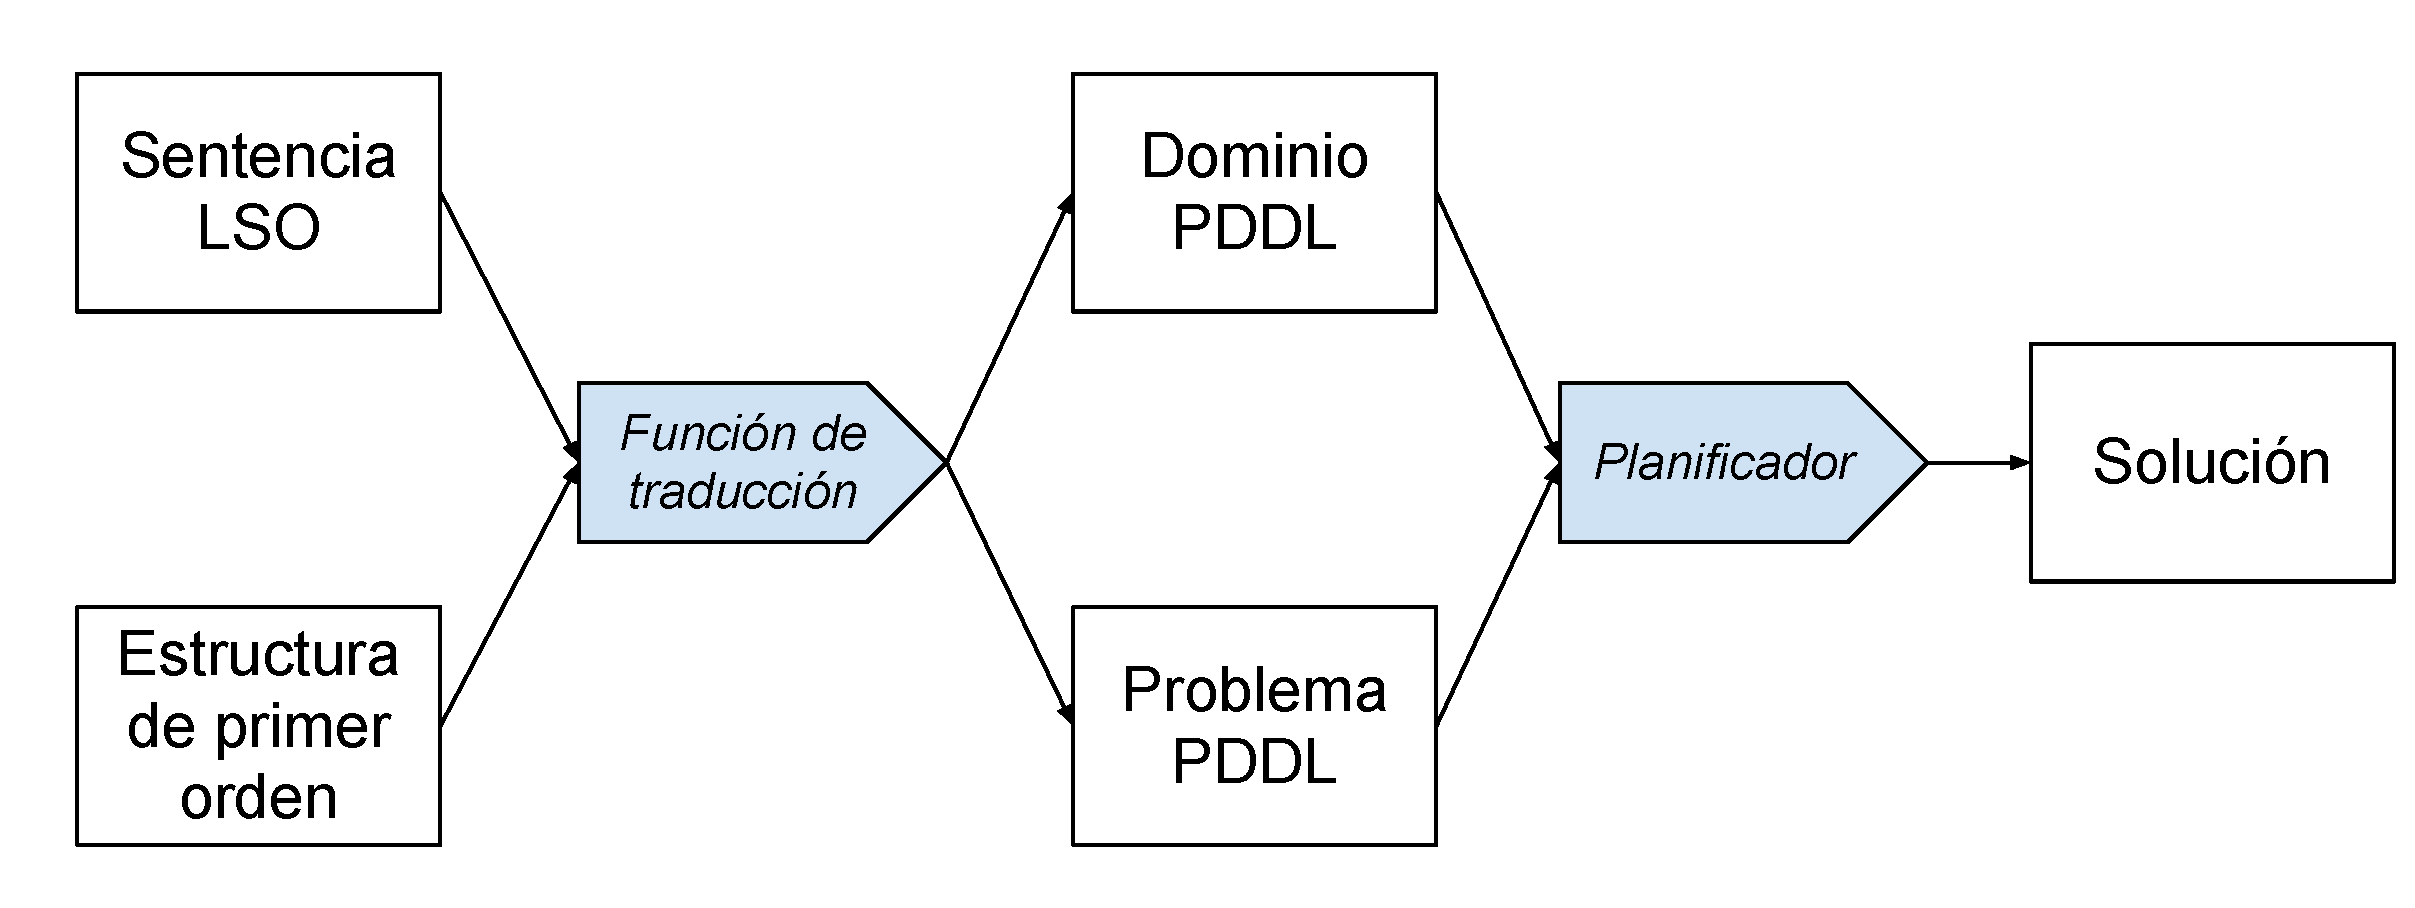
\includegraphics[width=\textwidth]{figuras/esquema_herramienta.pdf}
\caption{Esquema de operación de la herramienta}
\label{esquema_herramienta}
\end{figure}

\section{Diseño del lenguaje}

\subsection{Gramática}
\begin{alignat*}{1}
\sofbf\   & \deriv\ \lpar \SOExists\ \lpar \listrel \rpar\ \sofbf \rpar \\
          & \deriv\ \lpar \SOForall\ \lpar \listrel \rpar\ \sofbf \rpar \\
          & \deriv\ \pofbf \\[1em]
\listrel\ & \deriv\ \rel\ \integer\ \listrel\ |\ \rel\ \integer \\
          & \deriv\ \rel\ \tipof\ \listrel\ |\ \rel\ \tipof\ \\[1em]
\tipof\   & \deriv\ \fun\ |\ \pfun\ |\ \inj\ |\ \pinj\ \\[1em]
\pofbf\   & \deriv\ \lpar \rel\ \listvar \rpar \\
          & \deriv\ \lpar \NOT\ \pofbf \rpar \\
          & \deriv\ \lpar \AND\ \listpofbf \rpar \\
          & \deriv\ \lpar \OR\ \listpofbf \rpar \\
          & \deriv\ \lpar \IMPLIES\ \pofbf\ \pofbf \rpar \\
          & \deriv\ \lpar \Exists\ \lpar \listvar \rpar\ \pofbf \rpar \\
          & \deriv\ \lpar \Forall\ \lpar \listvar \rpar\ \pofbf \rpar \\[1em]
\listvar\ & \deriv\ \var\ \listvar\ |\ \var \\[1em]
\end{alignat*}

\section{Reducción base}
\subsection{Reducción del dominio}
\subsection{Reducción del problema}

\section{Propiedades formales}
Las propiedades más importantes a considerar en la herramienta son solidez,
completitud y garantía de complejidad. Que la función de traducción sea sólida
y completa significa que ella realmente implementa una reducción entre problemas de
decisión, mientras que la garantía de complejidad se refiere al tiempo
requerido para computar la reducción y la complejidad de decidir la existencia
de un plan en el problema generado. En esta sección se demuestra que la 
herramienta es una reducción en tiempo
polinomial del problema NP expresado por $\Phi$ a un fragmento de planificación
que es decidible en NP.

Como se ha mencionado en la sección \ref{complejidad_planificacion}, 
se sabe que verificar la existencia de un plan para 
problemas de planificación
sin efectos negativos está en NP \citep{bylander:plan-complexity}. La prueba
depende del hecho de que un plan óptimo no necesita repetir acciones, y por lo
tanto es de tamaño lineal. Puede extenderse esta noción: si todas las acciones que
agregan efectos negativos pueden ser aplicadas a lo sumo una vez, verificar la
existencia de un plan sigue estando en NP, pues el tamaño del plan no podrá ser
mayor al número de acciones.

\begin{definition}
Un problema de planificación $P = \tup{C, A, I, F}$ es de tipo
\textit{máximo-1} si y sólo si las acciones pueden ser particionadas en $A =
A_0 \cup A_1$, donde:
\begin{itemize}
\item Ninguna de las acciones de $A_0$ tiene efectos negativos, es decir,
$(\forall a \in A_0) (del(a) = \emptyset)$.
\item Todas las acciones de $A_1$ tienen una precondición que no es añadida por
ninguna acción, y que es borrada apenas $a$ es ejecutada, es decir, 
$(\forall aa' \in A_1)\ (\exists p \in pre(a) \cap del(a))\ (p \not\in add(a'))$
\end{itemize}

El conjunto de todos los problemas \textit{máximo-1} se denota como STRIPS-1.
\end{definition}

%! ???
Ahora considere la función de \emph{instanciación} $\ground$ que transforma el par
$\tup{\domain,\instance}$ de un dominio y problema PDDL en un problema STRIPS
$P = \ground(\domain, \instance)$. Para un $\domain$ fijo, la función
$\instance\leadsto\ground(\domain, \instance)$ corre en un tiempo polinomial
$\O(\|\instance\|^k)$ para algún $k$ que sólo depende de $\domain$; de hecho,
$k$ es la máxima aridad de un predicado o acción en el dominio.

De manera similar, la función de traducción $\insred$ corre en tiempo
polinomial en el tamaño de la estructura $\A$, pero exponencial sobre la aridad
más grande de un cuantificador de segundo orden existencial en $\Phi$. De este
modo, la función $f_{\sigma,\Phi}:\struc[\sigma]\rightarrow\text{STRIPS}$
definida por 
\[ f_{\sigma,\Phi}(\A) = \ground(\domred(\sigma,\Phi),\insred(\sigma,\Phi,\A)) \]
es una función en tiempo polinomial que asigna a las $\sigma$-estructuras un
problema instanciado STRIPS. Esta función es una reducción, tal como es
demostrado por

\begin{theorem}
\label{t1}
Sean $t_1,...,t_n$ términos instanciados, es decir, que no contienen
variables.\\
\mbox{\hspace{5mm} $(A, i[x:=u]) \models \varphi(t_1,...,t_n,x)$}\\
$\iff \tup{\text{si $a$ es una constante tal que } a^\A = u}$\\
\mbox{\hspace{5mm} $(A, i[x:=u]) \models \varphi(t_1,...,t_n,a)$}\\
$\iff \tup{\text{?}}$\\
\mbox{\hspace{5mm} $(A, i) \models \varphi(t_1,...,t_n,a)$}\\
\end{theorem}
\begin{lemma}
Sean $t_1,...,t_n$ términos instanciados y sea $a$ una constante. Sea $\A$ una
estructura tal que $u \in |\A|$, $a^\A = u$. Entonces:\\
\mbox{\hspace{5mm} $(A, i[x:=u]) \models \varphi(t_1,...,t_n,x)$}\\
$\iff \tup{a^\A = u}$\\
\mbox{\hspace{5mm} $(A, i[x:=u]) \models \varphi(t_1,...,t_n,a)$}\\
$\iff \tup{\text{?}}$\\
\mbox{\hspace{5mm} $(A, i) \models \varphi(t_1,...,t_n,a)$}\\
\end{lemma}


\begin{theorem}
La función $f_{\sigma, \Phi}$ es una reducción en tiempo polinomial del
problema de decisión inducido por $\Phi$ a STRIPS-1.
\end{theorem}

\begin{proof}
Se quiere demostrar que
$\A\models(\exists R_1^{a_1})\cdots(\exists R_k^{a_k})\psi$ si y sólo si
existe un plan que consigue la condición $\FT[\psi]$. La prueba es inductiva
sobre la estructurda de la sentencia de primer orden $\psi$. Se demostrará que para toda subformula 
$\theta$ de $\psi$, y toda interpretacion $(\A,i)$ de $\A$:

\[ (\A,i) \models \theta(\overline{X}) \iff \text{existe un plan para } \FT[\theta](\overline{X}) \]

Por implicación mutua. Primero se prueba
\[ (\A,i) \models \theta(\overline{X}) \Rightarrow \text{existe un plan para } \FT[\theta](\overline{X}) \]

\begin{center}
\begin{tabular}{ll}
\multicolumn{2}{l}{Caso base: $\theta$ es un literal, $\theta = R(t_1,...,t_k)$}\\
\multicolumn{2}{l}{Caso $R \in \sigma$}\\
&$\A \models R(t_1,...,t_k)$\\
&$\Rightarrow (\A,i) \models R(t_1,...,t_k)$\\
&$\Rightarrow \tup{i(t_1),...,i(t_k) \in R^\A}$\\
&$\Rightarrow R^\A(i(t_1),...,i(t_k))$\\
&$\Rightarrow R^\A$ pertenece a init, La situacion inicial (Init) consiste
de fluents describiendo el valor de verdad de todas las relaciones en $\A$\\
&$\Rightarrow \text{El plan vacío es un plan para }\theta(t_1,...,t_n)$.\\
\multicolumn{2}{l}{Caso $R \not\in \sigma$??}\\
\end{tabular}
\end{center}

\begin{tabular}{ll}
\end{tabular}

\begin{itemize}
		\item Caso base: $\theta$ is a literal. $\theta = P(X)$ 
		
		Prueba por casos:
			\begin{itemize}
				\item Caso 0: $P(\overline{X})$ $\epsilon$ $\sigma$
				
				\begin{tabular}{@{}p{1mm}p{1mm}p{11cm}}	
						& & $\A \models P(\overline{X})$\\
						$\eq$ & & $<(A,i)$ es una interpretacion de $\A>$ \\
						& & $(A,i) \models P(\overline{X})$ \\
						$\eq$ & & $<$Definicion de interpretacion$>$\\
						& & $i(\overline{X})$ $\epsilon$ $P^{\A}$\\
						$\Rightarrow$ & & $<$ La situacion inicial (Init) consiste de fluents describiendo el valor de 
									  verdad de todas las relaciones en $\A$$>$\\
						& & $P(\overline{X})$ $\epsilon$ $Init$ \\
						$\eq$ & & $<$ Hy un plan de cero pasos para $\theta(\overline{x})>$\\
						& & $\FT[\theta](\overline{X})$ tiene solucion
					\end{tabular}
					
					
				\item Caso 1: $P(\overline{X})$ $\epsilon$ $\Phi$
				
					  Falta
			\end{itemize}
			
		\item Caso inductivo:
			\begin{itemize}
				\item Caso 0: $\theta = \neg P(\overline{X})$ (Como esta definido en el paper la negacion esta solo en los literales)
				
				\begin{tabular}{@{}p{1mm}p{1mm}p{11cm}}	
						& & $\A \models \neg P(\overline{X})$\\
						$\eq$ & & $<(A,i)$ es una interpretacion de $\A>$ \\
						& & $(A,i) \models \neg P(\overline{X})$ \\
						$\eq$ & & $<$Definicion de interpretacion$>$\\
						& & $i(\overline{X})$ $\epsilon$ ${\neg P}^{\A}$\\
						$\Rightarrow$ & & $<$ La situacion inicial (Init) consiste de fluents describiendo el valor de 
									  verdad de todas las relaciones en $\A$ (La negacion de un literal es tomado como
									  un fluent nuevo)$>$\\
						& & $P(\overline{X})$ $\epsilon$ $Init$ \\ 
						$\eq$ & & $<$ Hy un plan de cero pasos para $\theta(\overline{x})>$\\
						& & $\FT[\theta](\overline{X})$ tiene solucion
				\end{tabular}
					
				\item Caso 1: $\theta = \psi \land \psi'$ (Logical And)
					  
					  Hipotesis inductiva:
					 	\begin{itemize}
					 		\item $(A,i) \models \psi \eq$ hay un plan para $\FT[\psi] = \pi$
							\item $(A,i) \models \psi' \eq$ hay un plan para $\FT[\psi'] = \pi'$
					 	\end{itemize}
				
					\begin{tabular}{@{}p{1mm}p{1mm}p{11cm}}	
					 	& & $\A \models \psi \land \psi'$\\
						$\eq$ & & $<(A,i)$ es una interpretacion de $\A>$ \\
						& & $(A,i) \models \psi \land \psi'$ \\
						$\eq$ & & $<$ Semantica de Primer orden $>$\\
						& & $(A,i) \models \psi \land (A,i) \models \psi'$ \\
						$\eq$ & & $<$Hipotesis inductiva$>$\\
						& & $\FT[\psi] = \pi \land \FT[\psi'] = \pi'$\\
						$\Rightarrow$ & & $<$ Operator $ prove\_and\_id >$\\
						& & $\FT[\theta](\overline{X})$ tiene solucion
					\end{tabular}
				\item Caso 2: $\theta = \psi \lor \psi'$ (Logical Or)
					  
					  Hipotesis inductiva:
					 	\begin{itemize}
					 		\item $(A,i) \models \psi \eq$ hay un plan para $\FT[\psi] = \pi$
							\item $(A,i) \models \psi' \eq$ hay un plan para $\FT[\psi'] = \pi'$
					 	\end{itemize}
				
					\begin{tabular}{@{}p{1mm}p{1mm}p{11cm}}	
					 	& & $\A \models \psi \lor \psi'$\\
						$\eq$ & & $<(A,i)$ es una interpretacion de $\A>$ \\
						& & $(A,i) \models \psi \lor \psi'$ \\
						$\eq$ & & $<$ Semantica de Primer orden $>$\\
						& & $(A,i) \models \psi \lor (A,i) \models \psi'$ \\
						$\eq$ & & $<$Hipotesis inductiva$>$\\
						& & $\FT[\psi] = \pi \lor \FT[\psi'] = \pi'$\\
						$\eq$ & & $<$ Operator $ prove\_or\_id$ twice, idempotencia del $\lor$ $>$\\
						& & $\FT[\theta](\overline{X})$ tiene solucion
					\end{tabular}
					
				\item Caso 3: $\theta = \exists x$ $ \psi(\overline{y},x)$ (Exists)
					  
					  Hipotesis inductiva:
					 	\begin{itemize}
					 		\item $(A,i) \models \psi(\overline{y},x)$ hay un plan $\pi$ para $\FT[\psi(\overline{y},x)] (\overline{y},x)$
					 	\end{itemize}
				
					\begin{tabular}{@{}p{1mm}p{1mm}p{11cm}}	
					 	& & $A \models \exists x$ $ \psi(\overline{y},x)$\\
						$\eq$ & & $<(A,i)$ es una interpretacion de $\A>$ \\
						& & $(A,i) \models \exists x$ $ \psi(\overline{y},x)$ \\
						$\eq$ & & $<$ Semantica de Primer orden $>$\\
						& & $(A,i) \models \psi(\overline{y},x)$ \\
						$\eq$ & & $<$Hipotesis inductiva$>$\\
						& & $\FT[\psi] = \pi \lor \FT[\psi'] = \pi'$\\
						$\eq$ & & $<$ Operator $ prove\_exists >$\\
						& & $\FT[\exists x$ $ \psi(\overline{y},x)](\overline{y})$ tiene solucion
					\end{tabular}

			\end{itemize}
		
	\end{itemize}
\end{proof}
